% !TEX program = xelatex
% =====================================================================
%  flico 期末報告主檔
%
%  編譯:
%    xelatex main.tex && biber main && xelatex main.tex && xelatex main.tex
%
%  圖檔來源:research-log/figures/<date>/ 與 ../simulation/figures/
%  (透過 \graphicspath 掛進來,不複製。)
% =====================================================================
\documentclass[12pt,a4paper]{article}

% ---- 版面 ----------------------------------------------------------
\usepackage[margin=1in]{geometry}
\usepackage{setspace}
\onehalfspacing
\usepackage{titling}
\setlength{\droptitle}{-1.5cm}
\usepackage{fancyhdr}
\setlength{\headheight}{15pt}
\pagestyle{fancy}\fancyhf{}
\renewcommand{\headrulewidth}{0.4pt}
\lhead{\leftmark}\rhead{\thepage}
\parindent=24pt

% ---- 數學與符號 ----------------------------------------------------
\usepackage{amsmath,amsthm,amssymb,amsbsy,bm}
\usepackage{siunitx}

% ---- 圖、表 --------------------------------------------------------
\usepackage{graphicx}
\graphicspath{%
  {figures/}%
  {research-log/figures/2026-05-06/}%
  {research-log/figures/2026-05-12/}%
  {research-log/figures/2026-05-18/}%
  {../simulation/figures/}%
}
\usepackage{float}
\usepackage{subfig}
\usepackage{booktabs}
\usepackage{array}
\usepackage{multirow}
\usepackage{longtable}
\usepackage{enumitem}

% ---- 連結 ----------------------------------------------------------
\usepackage{xcolor}
\usepackage[unicode=true,pdfborder={0 0 0},bookmarksdepth=-1,
            colorlinks=true,linkcolor=blue!55!black,citecolor=blue!55!black,
            urlcolor=teal]{hyperref}

% ---- 參考文獻(biblatex + biber)----------------------------------
\usepackage[backend=biber,style=numeric,giveninits=true]{biblatex}
\addbibresource{references.bib}

% ---- 中文字型 ------------------------------------------------------
\usepackage{xeCJK}
\setCJKmainfont{TW-Kai}[AutoFakeBold=2.5, AutoFakeSlant=0.2]
\setCJKmonofont{TW-Kai}[AutoFakeBold=2.5, AutoFakeSlant=0.2]
\setCJKsansfont{TW-Kai}[AutoFakeBold=2.5, AutoFakeSlant=0.2]

% =====================================================================
\title{\bfseries flico \\[4pt]
       \large 以 Raspberry Pi Pico 為核心的螢幕 / 光源閃爍量測儀\\[2pt]
       \normalsize {\it flicker meter} \(=\) BPW34 \(+\) MCP6004 TIA \(+\) Raspberry Pi Pico}
\author{Polarbear\\ \normalsize 國立臺灣大學}
\date{2026 年 6 月 7 日}

\begin{document}
\maketitle
\thispagestyle{fancy}

% =====================================================================
\begin{abstract}
  \noindent\textbf{flico}(\textit{flicker} \(+\) \textit{pico})是一台以
  \textbf{Raspberry Pi Pico} 為核心、自製的螢幕 / 光源閃爍(flicker)量測儀。
  光訊號由 Vishay \textbf{BPW34} 矽 PIN 光二極體接收,經 Microchip
  \textbf{MCP6004} 跨阻放大器(TIA,transimpedance amplifier)轉成電壓,
  由 Pico 內部 12-bit ADC 取樣後,一路透過 USB-CDC 串列傳到桌面端的 \textbf{Rust GUI}
  即時繪出時域波形與 FFT 頻譜,另一路由 0.91 吋 I\textsuperscript{2}C OLED
  獨立顯示瞬時電壓。

  \medskip
  本份報告對應的硬體狀態是\textbf{送 JLCPCB 製版之前的麵包板原型}:
  MCP6004(只用其中一個 op-amp)\(+\) 74HC4051 8 通道類比 mux(只啟用 4 個通道)
  \(+\) 4 檔 gain(\(R_f \in \{\SI{1}{\kilo\ohm}, \SI{10}{\kilo\ohm},
  \SI{100}{\kilo\ohm}, \SI{1}{\mega\ohm}\}\))。\textbf{4 檔 \(R_f C_f\) 乘積
  全部對齊成 \SI{10}{\micro\second}},使各檔截止頻率\textbf{一致}收斂到
  \(f_c \approx \SI{16}{\kilo\hertz}\)。整套裝置的物料成本約\textbf{新台幣 435 元},
  證明「自己動手做光學儀器」在大學專題層級是可行的。報告最後說明已送製、
  仍在運送途中的 PCB 版規格升級路線:\textbf{OPA320 \(+\) TMUX1208 \(+\) 8 檔
  \(R_f\) (\(\SI{10}{\ohm}\) 到 \(\SI{100}{\mega\ohm}\)) \(+\) SFH 2440
  類人眼光譜光二極體 \(+\) 3D 列印整機外殼}。
\end{abstract}

% =====================================================================
\section{前言:為什麼要量「看不見的閃」}

人眼對閃爍的敏感頻段約在 \(\SIrange{3}{60}{\hertz}\) 之間,但現代螢幕 / LED 燈具
普遍以 \(\SI{100}{\hertz}\)(電源整流頻率 \(\times 2\))到 \(\SI{25}{\kilo\hertz}\)
之間的 PWM 調光,看似「不會閃」其實仍有強度週期性變化\,\cite{IEEE1789}。
這種\textbf{次感知頻段的閃爍}已被 IEEE Std 1789-2015 列為潛在的視覺疲勞、
偏頭痛、誘發癲癇風險來源。flico 的目的就是\textbf{把人眼看不見的閃變成桌面 GUI
上看得見的曲線}。

設計目標:

\begin{itemize}[leftmargin=2em,itemsep=0pt]
  \item \textbf{頻寬至少 \SI{16}{\kilo\hertz}}:涵蓋 IEEE 1789 關注的 \(\leq\)
        \SI{12.5}{\kilo\hertz} 範圍,並留一些 margin。
  \item \textbf{動態範圍跨 4 個數量級的入射光強度}:從暗室到日光皆要量得到 \\
        \(\to\) 用 \textbf{多檔 \(R_f\) 跨 \(10^3 \times\) 增益}解。
  \item \textbf{單機可獨立顯示瞬時亮度},接上電腦才開 FFT 詳查 \\
        \(\to\) 用 I\textsuperscript{2}C OLED 補上輕量化的「離線模式」。
  \item \textbf{總材料費控制在新台幣 500 元以下},
        當作大學專題層級的「\textbf{自製儀器}」demonstrator。
\end{itemize}

% =====================================================================
\section{系統概觀}

訊號鏈如圖~\ref{fig:signal-chain} 所示,共 5 級:

\begin{equation*}
  \text{光} \;\to\; \text{BPW34 PD} \;\to\; \text{MCP6004 TIA} \;\to\;
  \text{74HC4051 MUX} \;\to\; \text{Pico ADC \(+\) USB-CDC} \;\to\;
  \text{Rust GUI \(/\) OLED}
\end{equation*}

\begin{figure}[H]
  \centering
  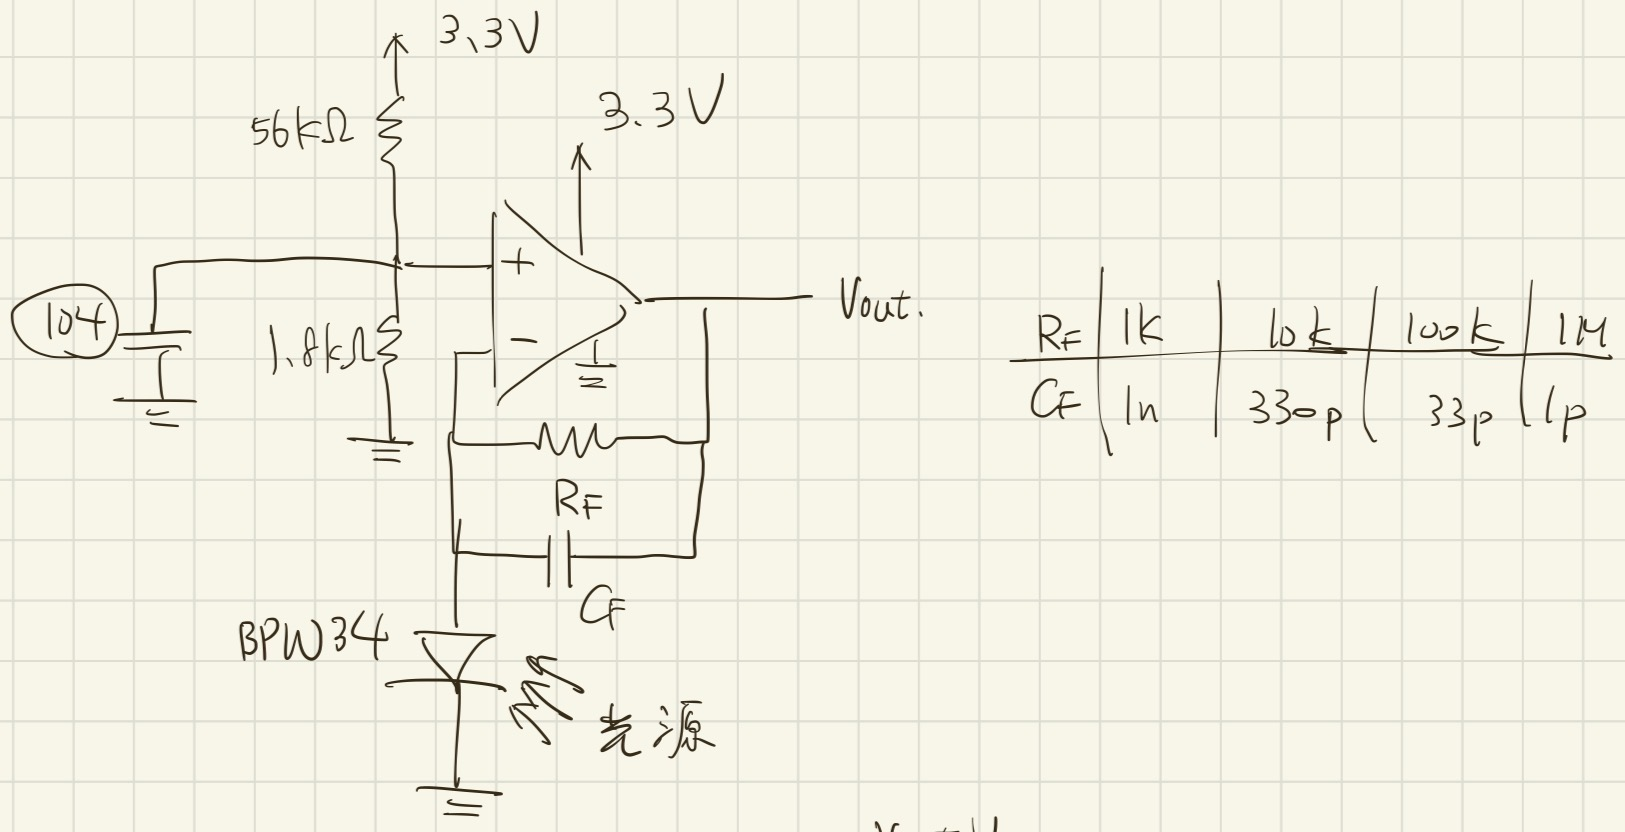
\includegraphics[width=0.85\linewidth]{initial_schmatic.jpg}
  \caption{flico 初版手繪電路:BPW34 直接接 MCP6004 反相端,
    回授支(\(R_f \parallel C_f\))由 74HC4051 8 通道 mux 選檔。本檔已實作為麵包板原型。}
  \label{fig:signal-chain}
\end{figure}

每一級的選型與權衡列於表~\ref{tab:bom-current}。

\begin{table}[H]
  \centering
  \caption{flico 麵包板版主要零件清單與選型理由。}
  \label{tab:bom-current}
  \small
  \begin{tabular}{lll}
    \toprule
    元件        & 型號                       & 選型理由 \\
    \midrule
    光二極體    & Vishay \textbf{BPW34}      & 大面積(\SI{7.5}{\milli\meter\squared}),
                                              敏感波段 \SIrange{430}{1100}{\nano\meter},
                                              台灣容易買、便宜\,\cite{BPW34Datasheet} \\
    跨阻放大器  & Microchip \textbf{MCP6004} & 單電源 3.3\,V 可跑、軌到軌輸出、
                                              \SI{1}{\mega\hertz} GBW;
                                              4 op-amp 但本版只用 1 個\,\cite{MCP6004Datasheet} \\
    類比 MUX    & \textbf{74HC4051}          & 8 通道,3 條 select 線即可定址;
                                              本版只用 4 通道\,\cite{HC4051Datasheet} \\
    MCU         & \textbf{Raspberry Pi Pico} & 內含 12-bit ADC \(\times\) 3,
                                              USB-CDC 直接出訊號,3.3\,V 邏輯\,\cite{PicoDatasheet} \\
    顯示器      & 0.91" I\textsuperscript{2}C OLED & \(128 \times 32\) dot,
                                                    SSD1306 控制器,
                                                    Pico 端用 GP4/GP5 走 I\textsuperscript{2}C \\
    \bottomrule
  \end{tabular}
\end{table}

% =====================================================================
\section{電路設計(麵包板版)}
\label{sec:circuit}

\subsection{TIA 拓樸:讓光二極體跑在零偏壓}

BPW34 接在 MCP6004 的反相輸入端,正輸入端接 \(V_{cc}/2 = \SI{1.65}{\volt}\)
(由 Pico 3.3\,V 經兩顆等值電阻分壓,再用 \SI{0.1}{\micro\farad} 旁路)。
op-amp 的虛短特性讓 PD 兩端電壓近乎為零,\textbf{光電流 \(I_{pd}\)
完全流過回授阻抗 \(Z_f = R_f \parallel C_f\)},輸出電壓:

\begin{equation}
  V_\text{out}(s) = V_{cc}/2 \;-\; I_{pd}(s) \cdot \frac{R_f}{1 + sR_fC_f}.
  \label{eq:tia-tf}
\end{equation}

零偏壓\((V_R \approx 0)\) 是\textbf{刻意選擇}:相較於逆偏(會壓低 PD 寄生電容、
拉高頻寬),零偏壓的暗電流低 \(\sim 3\) 個數量級,在量\textbf{深暗環境下的低頻
flicker}(例如手機 OLED 最低亮度 PWM)時 SNR 明顯較好。代價是 PD 寄生電容
\(C_{pd} \approx \SI{70}{\pico\farad}\) 較大,需要在 \(C_f\) 上做穩定性補償
(見下節)。

\subsection{巧思 1:4 檔 gain 共用同一截止頻率}
\label{sec:gain-table}

flico 麵包板版開了 4 檔 gain,涵蓋 \(10^3 \times\) 動態範圍。\textbf{關鍵的設計
巧思在於:每一檔的 \(R_f \times C_f\) 乘積都刻意拼成 \SI{10}{\micro\second}},
讓\textbf{所有檔位共用同一個 \(\sim \SI{16}{\kilo\hertz}\) 截止頻率},
換檔只是換增益、不換頻寬。

代入 \(f_c = 1/(2\pi R_f C_f)\):

\begin{equation}
  R_f C_f = \frac{1}{2\pi f_c} = \frac{1}{2\pi \times \SI{16}{\kilo\hertz}}
  = \SI{9.95}{\micro\second} \approx \SI{10}{\micro\second}.
  \label{eq:rc-product}
\end{equation}

四檔配對如表~\ref{tab:gain-current}。

\begin{table}[H]
  \centering
  \caption{麵包板版 4 檔 gain 配對。\(R_f C_f\) 全部等於 \SI{10}{\micro\second},
    對應 \(f_c \approx \SI{16}{\kilo\hertz}\)。}
  \label{tab:gain-current}
  \begin{tabular}{cllll}
    \toprule
    通道 & \(R_f\)         & \(C_f\) (SMD 標印)    & 跨阻增益           & 適用入射光 \\
    \midrule
    0    & \SI{1}{\kilo\ohm}    & \SI{10}{\nano\farad} (\texttt{103})    & \(10^3\,\text{V/A}\) & 強光(室內 \(>\)\SI{1000}{lx}) \\
    1    & \SI{10}{\kilo\ohm}   & \SI{1}{\nano\farad} (\texttt{102})     & \(10^4\,\text{V/A}\) & 中等光(辦公室常見) \\
    2    & \SI{100}{\kilo\ohm}  & \SI{100}{\pico\farad} (\texttt{101})   & \(10^5\,\text{V/A}\) & 弱光(臥室夜間) \\
    3    & \SI{1}{\mega\ohm}    & \SI{10}{\pico\farad} (\texttt{100})    & \(10^6\,\text{V/A}\) & 暗室 \(/\) 手機 OLED 最低亮度 PWM \\
    \bottomrule
  \end{tabular}
\end{table}

\textbf{為什麼這件事很重要?} 一般初學者的多檔 TIA 設計只切換 \(R_f\)、不動 \(C_f\),
結果各檔截止頻率隨 \(R_f\) 變動 \(3\) 個數量級——換一次檔,頻譜的「可信範圍」
就要跟著重畫,FFT 的 \(x\) 軸沒辦法跨檔比較。flico 把 \(C_f\) 也一起換進 mux,
\textbf{付出的代價只是多 4 顆陶瓷電容(每顆 NT\$\,2)},得到的好處是\textbf{換檔
不破壞頻譜量測的物理意義},FFT 圖在四檔之間可以直接疊上去比。

\subsection{巧思 2:用 mux 把波段開關吃掉}

回授支從 op-amp 的反相端拉出來,接到 \textbf{74HC4051 的 common 腳(\texttt{COM})},
4 條通道(\texttt{Y0}\(\sim\)\texttt{Y3})各接一組 \(R_f \parallel C_f\)\(\to\)
共同接回 op-amp 輸出。Pico 用 GP10/GP11/GP12 三條腳當 mux select 線(本版
最高位 \texttt{S2} 永遠拉低,因為只用 4 通道),按一下實體按鍵就升一檔、降一檔。

\textbf{設計上的細節}:

\begin{itemize}[leftmargin=2em,itemsep=0pt]
  \item 74HC4051 的 \(R_\text{on} \approx \SI{70}{\ohm}\) 跟最小檔 \(R_f =
        \SI{1}{\kilo\ohm}\) 是 \(7\%\) 誤差,\textbf{會直接污染最大電流檔的增益讀數};
        本版選擇\textbf{接受並在韌體端做查表校正},未來 PCB 版會換成
        \(R_\text{on} \approx \SI{5}{\ohm}\) 的 TMUX1208PW(\(0.5\%\) 誤差)。
  \item mux 切換瞬間會有 \(\sim \SI{100}{\nano\second}\) 的 break-before-make
        死區,輸出會跳一下;韌體在切檔後\textbf{丟掉前 5 個 ADC 樣本}避開突波。
\end{itemize}

\subsection{電源 \(+\) 麵包板實作}

整個 analog 走 Pico 內建的 3V3\_OUT(從 Pico 的 SMPS 經 SBU 出來的 \(\sim
\SI{300}{\milli\volt_{pp}}\) 噪音\(3.3\,V\) 軌),經 \SI{10}{\micro\farad}
鉭電容旁路後當 \(V_{cc}\)。\textbf{已知這條軌不乾淨}——5/12 在示波器上量到
明顯的 \SI{20}{\kilo\hertz} 來自 Pico SMPS 開關噪音——但麵包板級別只能容忍
這個級別,PCB 版會走 LP5907 LDO \(+\) ferrite bead 的乾淨類比 3.3\,V 軌
(已在 \texttt{hardware/final-version/SOC\_Final.kicad\_sch} 內實作)。

實際麵包板布局與焊接照片見圖~\ref{fig:breadboard},麵包板版的「半成品」
完整訊號鏈展示。

\begin{figure}[H]
  \centering
  \subfloat[BPW34 焊上排針的近照(5/12)]{%
    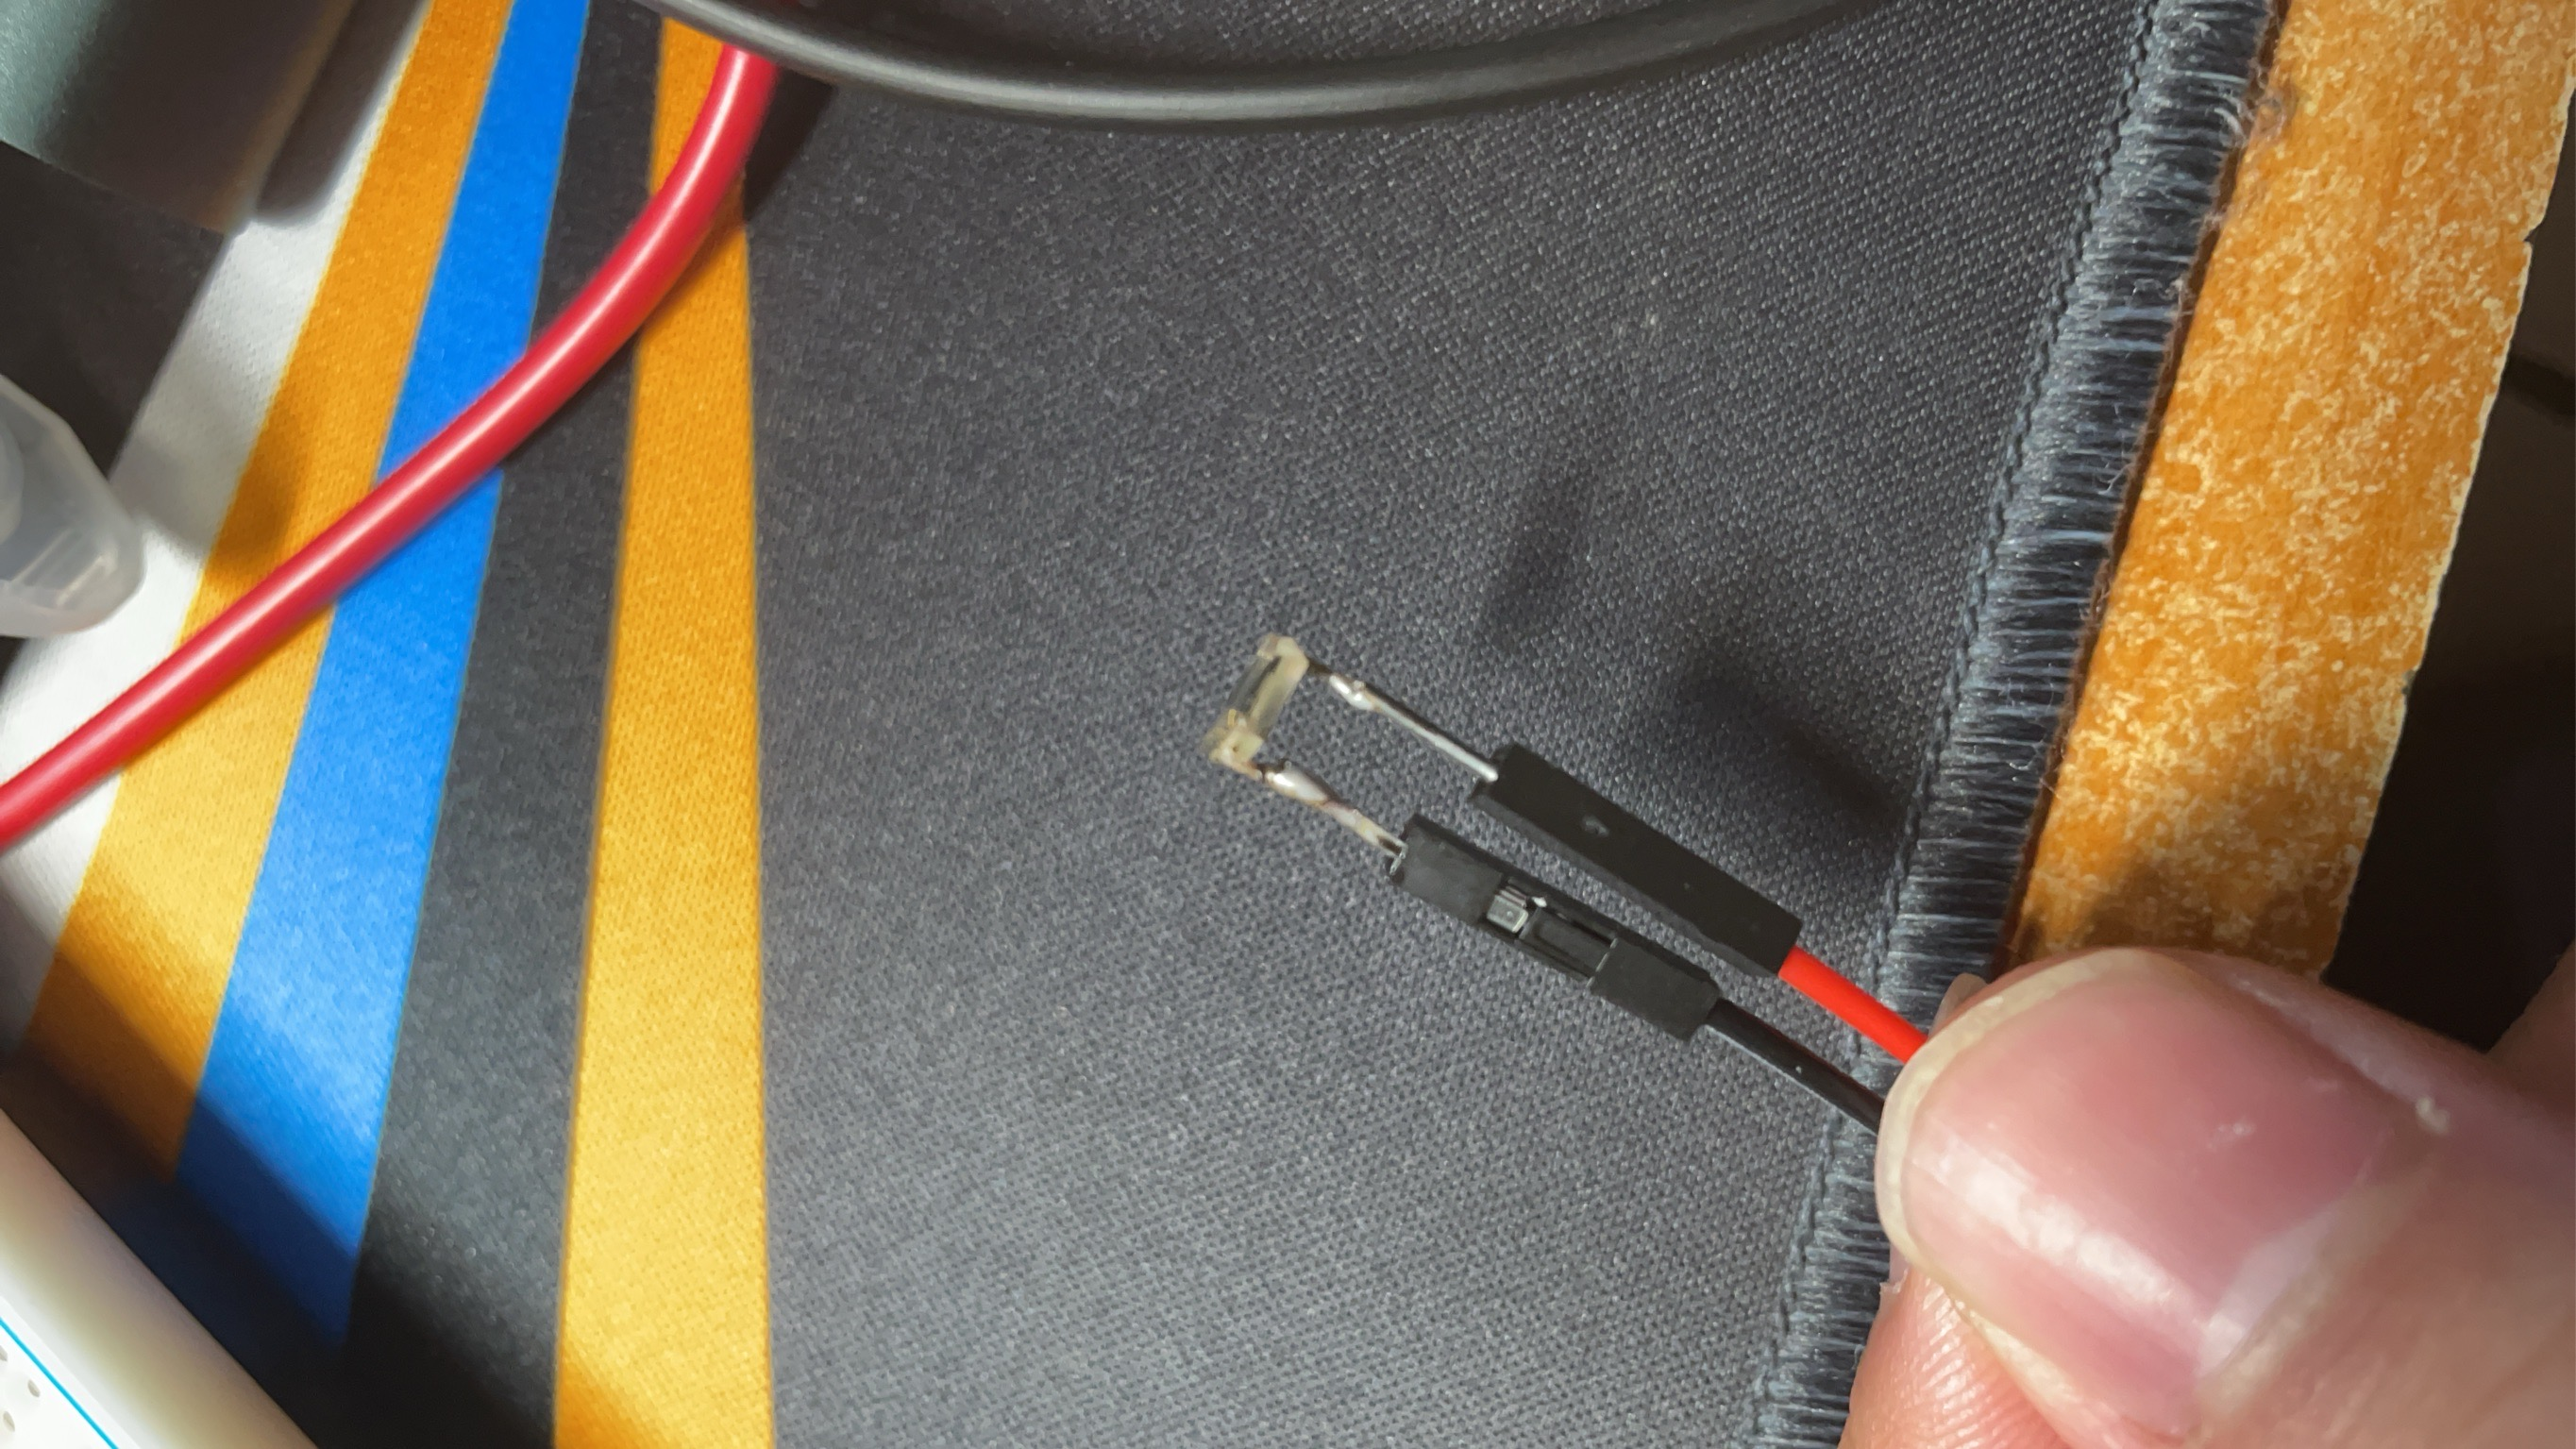
\includegraphics[height=4.5cm]{BPW34_solder.JPG}}\hfill
  \subfloat[最終定稿的麵包板電路圖手繪(5/12)]{%
    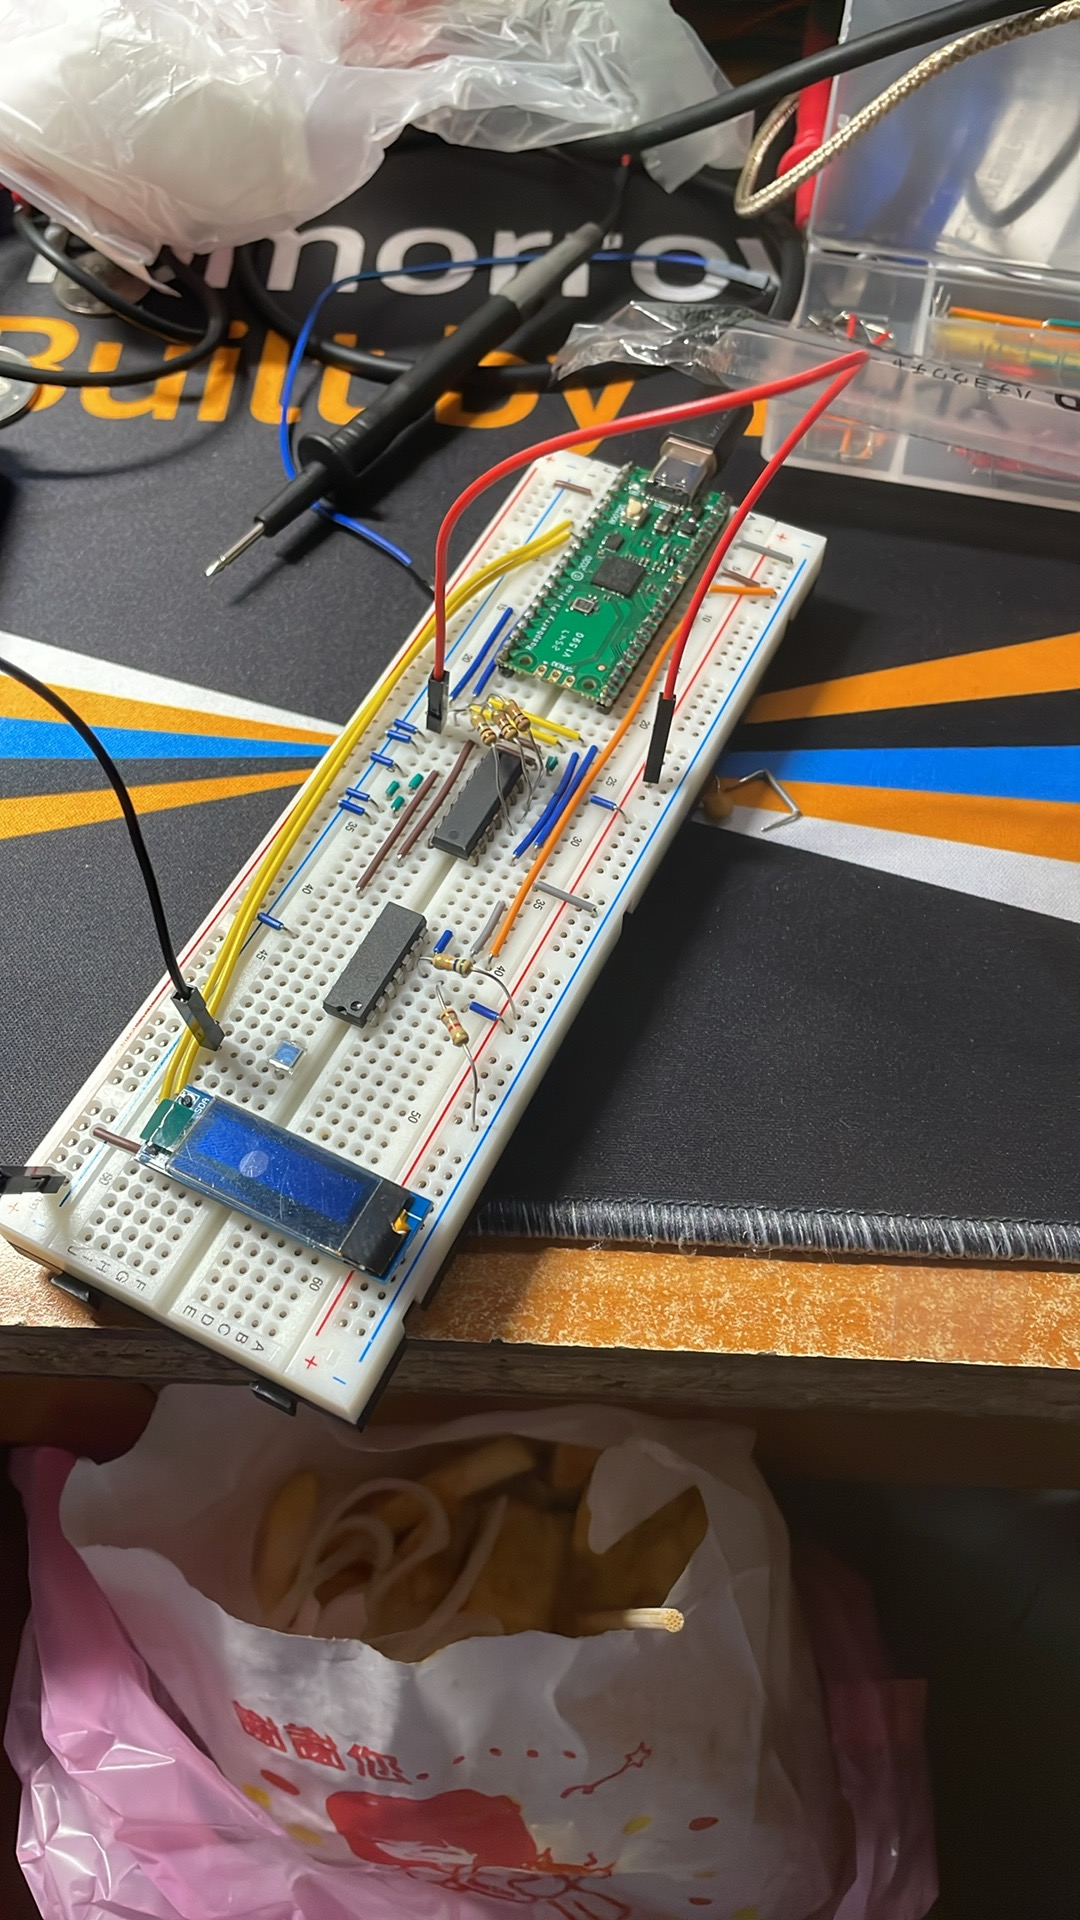
\includegraphics[height=4.5cm]{final_schmatic.JPG}}
  \caption{麵包板版實體與電路手稿。}
  \label{fig:breadboard}
\end{figure}

% =====================================================================
\section{韌體:C++ Pico SDK}

\subsection{為什麼從 MicroPython 改寫成 C++}

整個專案的韌體一開始是用 \textbf{MicroPython} 寫的(對應 \texttt{firmware/python-version/}),
因為 edit \(\to\) save \(\to\) run 的循環只要 1 秒,原型迭代最快。但測完發現:

\begin{itemize}[leftmargin=2em,itemsep=0pt]
  \item MicroPython 的 \texttt{adc.read\_u16()} 是純解譯式呼叫,單樣本要 \(\sim
        \SI{40}{\micro\second}\)。\textbf{採樣率被卡在 \SI{25}{\kilo\hertz}},
        剛好不能可靠抓到 \SI{16}{\kilo\hertz} 的訊號(Nyquist 要 \(2 \times\) 還
        要留 margin)。
  \item I\textsuperscript{2}C OLED 更新一個 frame 要 \(\sim \SI{30}{\milli\second}\),
        在這個 \(30\,\text{ms}\) 區間 ADC 採樣會\textbf{完全暫停},時域曲線會出現
        週期性的「\textbf{破洞}」。
\end{itemize}

5/12 整天 fork 出 \textbf{C++ Pico SDK} 版,直接呼叫 RP2040 的 ADC 硬體:
\texttt{adc\_select\_input(0); adc\_read();} 單樣本 \(\sim \SI{2}{\micro\second}\),
採樣率輕鬆拉到 \SI{500}{\kilo\hertz}(實際本版設 \SI{50}{\kilo\hertz} 留 margin)。
OLED 更新改放在獨立的 timer ISR、每 \SI{200}{\milli\second} 刷一次,跟 ADC 採樣
互不干擾。

\subsection{韌體架構}

\texttt{firmware/cpp-version/} 的核心檔案:

\begin{itemize}[leftmargin=2em,itemsep=0pt]
  \item \texttt{main.cpp}:設定 ADC 通道 0(GP26)\(+\) USB-CDC 出口,
        進入 \texttt{while(true)} 主迴圈:
        \begin{enumerate}[leftmargin=2em,itemsep=0pt]
          \item 從 ADC 拉 1 樣本(\SI{12}{bit})
          \item 透過 \texttt{stdio\_usb} 推 3 byte binary frame
                (\texttt{[sync\_byte, high\_8bit, low\_4bit]})到 USB-CDC
          \item 檢查按鍵狀態 \(\to\) 必要時切 mux select 線
        \end{enumerate}
  \item \texttt{ssd1306.cpp / .hpp}:從 Pico SDK 範例改寫的純 C++ 驅動,
        實作 \texttt{init()}, \texttt{clear()}, \texttt{draw\_text()},
        \texttt{flush()}。一個 frame buffer 是 \(128 \times 32 / 8 = 512\) byte,
        I\textsuperscript{2}C 速率 \SI{400}{\kilo\hertz}。
\end{itemize}

\textbf{巧思}:3-byte binary frame 比 ASCII CSV 省 \(\sim 4 \times\) 頻寬,
USB-CDC 在 macOS 端用 Rust 解碼開銷可以忽略,讓 \SI{50}{\kilo\hertz} 採樣率
可以無遺漏地一路推到桌面 GUI。

% =====================================================================
\section{桌面 GUI(Rust)}

桌面 GUI 本版用 \textbf{Rust} \(+\) \textbf{eframe / egui} 撰寫,
crate 名 \texttt{rust\_flico},放在 \texttt{host/}。完整原始碼只有
一個 \texttt{src/main.rs}(\(\sim 1\,270\) 行)。

\subsection{為什麼從 Python 改寫成 Rust}

對應的 5/19 研究日誌寫了完整的痛點分析,這裡只摘要結論。Python 版走過
\textbf{兩階段失敗}:

\begin{itemize}[leftmargin=2em,itemsep=0pt]
  \item \textbf{matplotlib \(+\) \texttt{plt.ion()}}:macOS retina backend
        每次 redraw 整個 figure,在 \SI{60}{\hertz} 同步翻轉下\textbf{會閃},
        且 \(> 10^4\) 樣本 fps 掉到 \(\sim 8\)。
  \item \textbf{PyQtGraph (OpenGL backend)}:解掉閃但 \(> 3 \times 10^4\) 樣本
        fps 掉到 \(\sim 0.5\),根本原因是 NumPy \(\leftrightarrow\) Qt scene graph 的
        memcpy \(+\) Python GIL 跟 serial reader thread 互搶。
\end{itemize}

換 Rust 之後\textbf{單槍突破}:eframe 是 immediate-mode GUI,
\texttt{\&[f32]} 直推 GPU vertex buffer,沒有 retained scene graph 要維護;
序列讀取走 \texttt{std::thread} \(+\) \texttt{crossbeam-channel},\textbf{沒有 GIL}。

效能比較如表~\ref{tab:fps}(同一台 M1 Air,同樣的訊號)。

\begin{table}[H]
  \centering
  \caption{host 端三種繪圖技術在不同累積樣本數下的 fps 比較。}
  \label{tab:fps}
  \begin{tabular}{lrrr}
    \toprule
    累積樣本數                & matplotlib & PyQtGraph                & Rust (egui\_plot) \\
    \midrule
    \(10^3\)                  & 20         & 60                       & 60(V-sync 上限) \\
    \(10^4\)                  & 8          & 60                       & 60 \\
    \(3 \times 10^4\)         & 3          & 0.5                      & 60 \\
    \(10^5\)                  & 1          & 卡死                     & 40 \\
    \(3 \times 10^5\)         & 卡死        & 卡死                     & 30 \\
    \bottomrule
  \end{tabular}
\end{table}

\subsection{GUI 主要功能}

\begin{itemize}[leftmargin=2em,itemsep=0pt]
  \item \textbf{時域 \(\leftrightarrow\) FFT 連動 zoom}:時域圖的 \(x\) 軸視窗
        改變時自動送新的 \texttt{FftJob}, FFT panel 顯示\textbf{該視窗區間的頻譜},
        而不是整段累積資料的頻譜。
  \item \textbf{Auto-detect Pico port}:macOS 掃 \texttt{/dev/cu.usbmodem*},
        Windows 預設 \texttt{COM3}。
  \item \textbf{CSV export}:\texttt{flicker\_<unix\_ts>.csv} 一鍵存,做後續分析。
  \item \textbf{Synth mode}:\texttt{--synth} flag 跑合成 sinusoid \(+\) noise,
        demo 時不用接實體 Pico。
  \item \textbf{WASM target}:\texttt{cargo build --target wasm32-unknown-unknown}
        產出 \(\sim \SI{8}{MB}\) \texttt{.wasm},可直接丟瀏覽器展示
        (sample source 限定 synth)。
\end{itemize}

% =====================================================================
\section{量測 vs 模擬交叉驗證}

5/6 在實作 TIA 之前,先用 \textbf{PySpice} 跑了完整的 DC sweep \(+\) AC Bode
\(+\) transient,確認電路在四檔下都穩定。模擬與量測結果如圖~\ref{fig:sim-meas}。

\begin{figure}[H]
  \centering
  \subfloat[DC sweep:不同 \(R_f\) 下 \(I_{pd} \to V_\text{out}\) 線性度]{%
    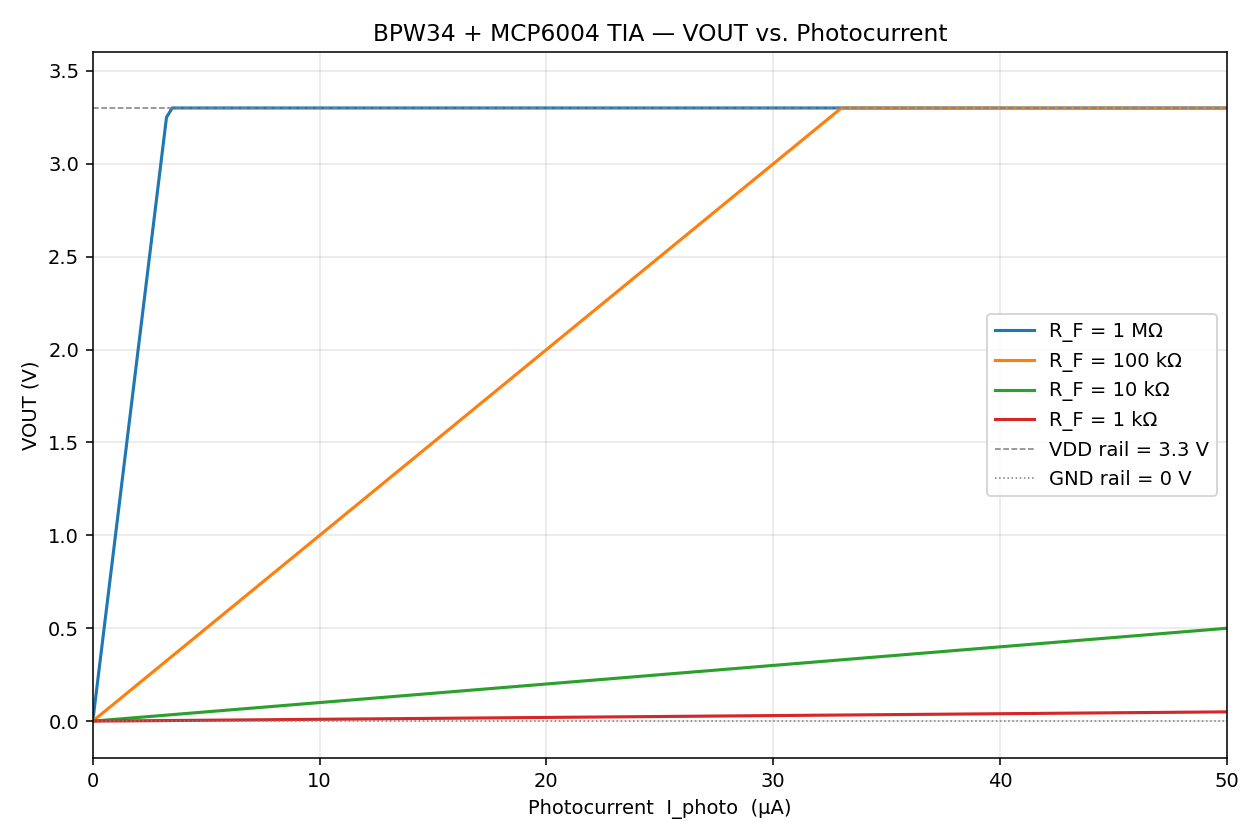
\includegraphics[width=0.31\linewidth]{tia_sweep.png}}\hfill
  \subfloat[AC Bode:四檔截止頻率\textbf{重合}於 \(\sim \SI{16}{\kilo\hertz}\)]{%
    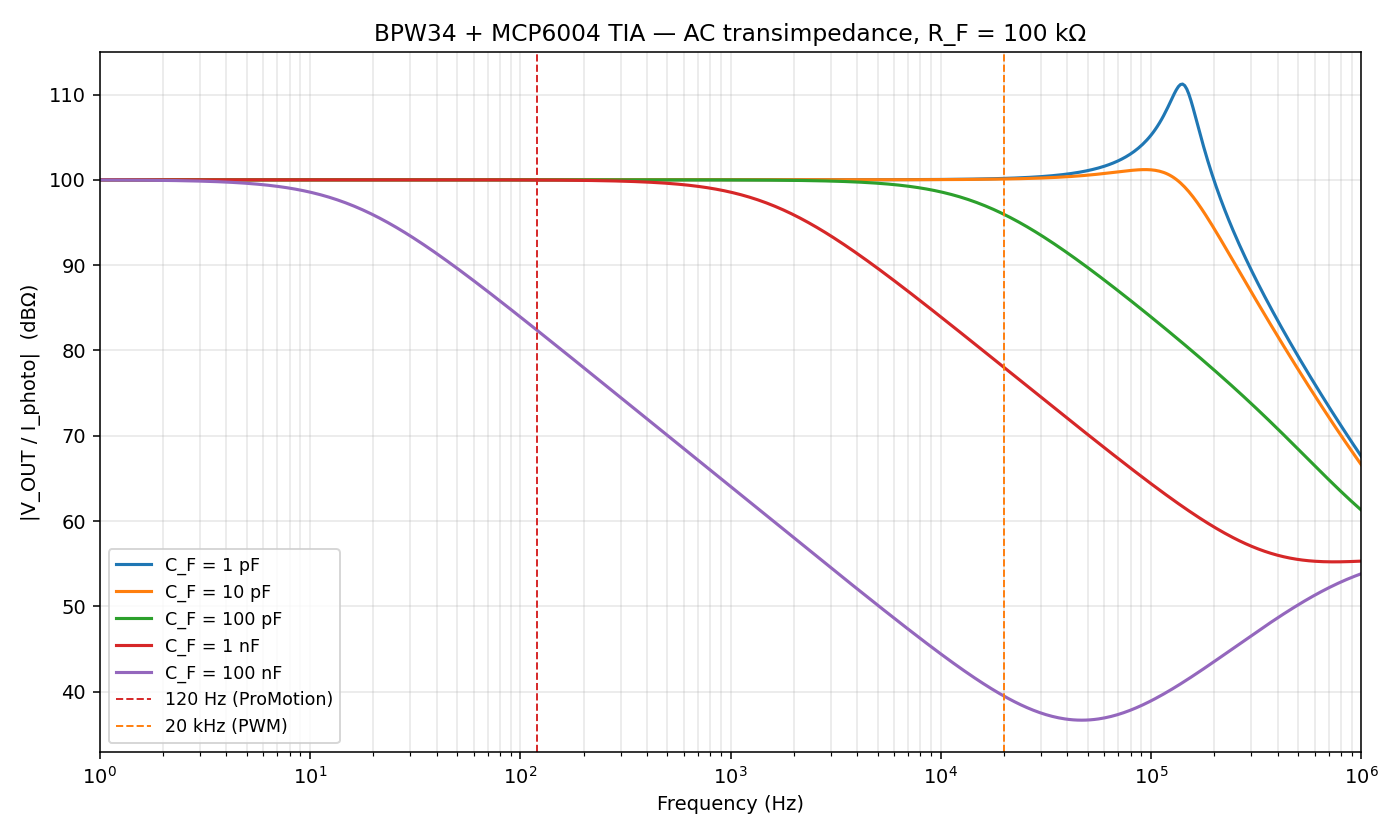
\includegraphics[width=0.31\linewidth]{ac_bode.png}}\hfill
  \subfloat[Transient:對 \SI{20}{\kilo\hertz} PWM 的響應]{%
    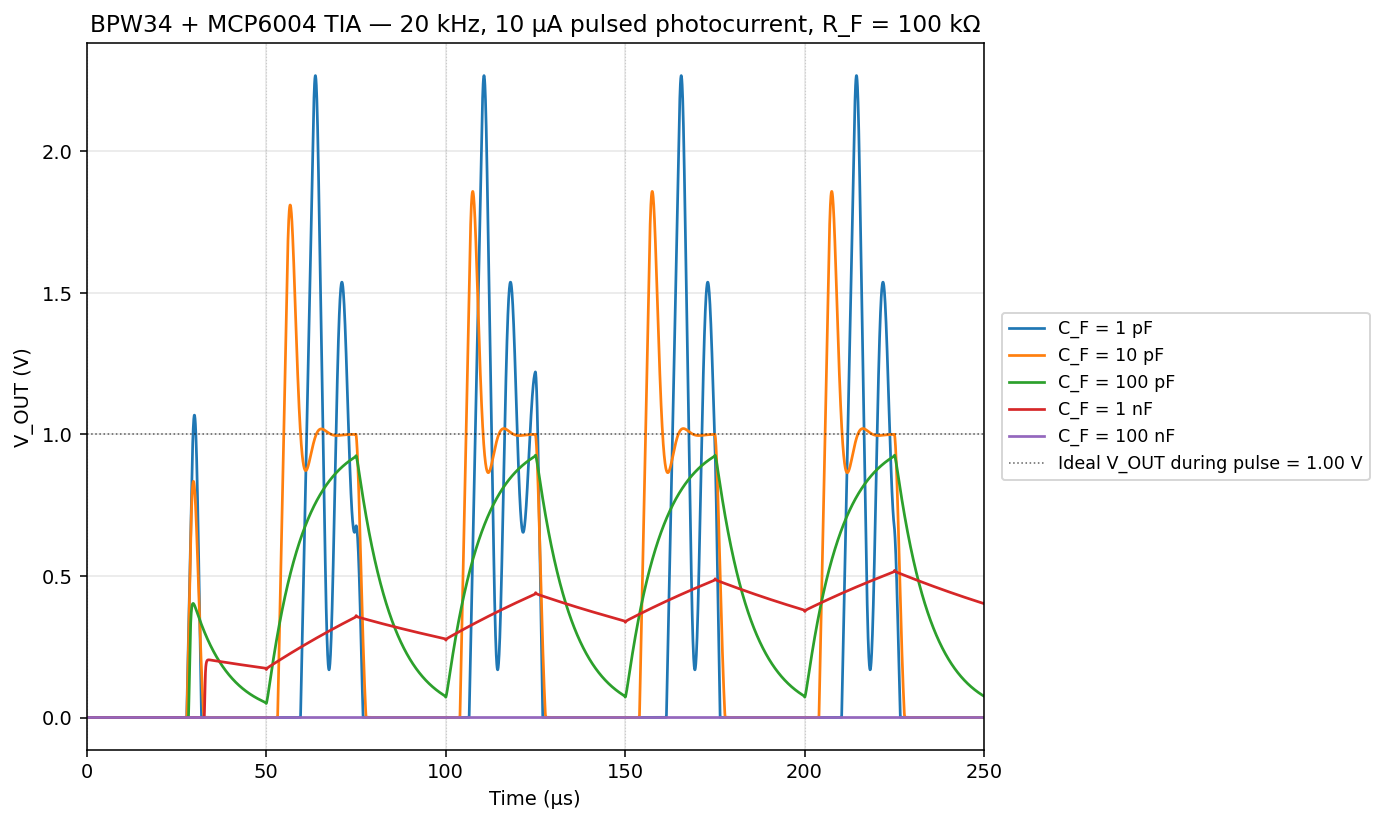
\includegraphics[width=0.31\linewidth]{transient_pwm.png}}
  \caption{PySpice 模擬結果。AC Bode 圖中四條曲線在 high-frequency 段
    \textbf{完全重合}——這是 \(R_f C_f\) 對齊設計的視覺證據。}
  \label{fig:sim-meas}
\end{figure}

\textbf{方法論巧思:實測噪音 \(\to\) PWL \(\to\) Spice}。
flico 不只「跑模擬」,還把 Rust GUI 量到的 BPW34 真實噪音(對著平面光源
量 \SI{8}{\second} 存成 CSV),透過 \texttt{host/convert.py} 轉成 KiCad
能讀的 PWL 噪音源,塞進 \texttt{hardware/final-version/TIA\_Gain\_100M.wbk}
spice 工作簿,讓\textbf{模擬的雜訊背景跟實體電路一致},而不是用人造白噪音湊。
這條 pipeline 是專案中最得意的方法論。

% =====================================================================
\section{造價}
\label{sec:cost}

表~\ref{tab:cost} 列出麵包板原型的零售價(2026 年 5 月台北光華電子實際採購)。

\begin{table}[H]
  \centering
  \caption{flico 麵包板版材料成本(新台幣)。}
  \label{tab:cost}
  \begin{tabular}{llrr}
    \toprule
    類別       & 項目                                  & 數量 & 小計 (NT\$) \\
    \midrule
    主動元件   & BPW34 光二極體                        & 1    & 25  \\
               & MCP6004 4 op-amp(只用 1)             & 1    & 30  \\
               & 74HC4051 8 通道 mux                   & 1    & 10  \\
               & Raspberry Pi Pico                     & 1    & 190 \\
    顯示       & 0.91" I\textsuperscript{2}C OLED (\(128 \times 32\))     & 1    & 80  \\
    被動元件   & 1/4\,W 電阻 (\SI{1}{\kilo\ohm} \(\sim\) \SI{1}{\mega\ohm}) & 4 & 4 \\
               & 陶瓷電容 (\SI{10}{\pico\farad} \(\sim\) \SI{10}{\nano\farad}) & 4 & 8 \\
               & \SI{10}{\micro\farad} 鉭電容(電源旁路) & 1    & 4   \\
               & 分壓電阻 \(\times\) 2 \(+\) \SI{0.1}{\micro\farad} 旁路   & 1 \text{組}    & 6 \\
    機構       & 半號麵包板                            & 1    & 50  \\
               & 跳線 \(+\) 公-母排針                  & 1 \text{組}    & 30  \\
    周邊       & USB Type-C 線(macOS 端)             & 1    & 0(自備) \\
    \midrule
    \multicolumn{3}{l}{\textbf{總計}}                                       & \textbf{435} \\
    \bottomrule
  \end{tabular}
\end{table}

對照市售 PWM 閃爍量測儀\(\sim \) NT\$\,5\,000\(\sim 30\,000\) 之間,
\textbf{本專案以 \(\sim 1/10\) 不到的成本做到了 \(\sim 16\) kHz 頻寬與
\(10^3 \times\) 動態範圍}。

% =====================================================================
\section{未來展望:PCB 版的規格升級路線}
\label{sec:future}

JLCPCB 製版包已於 2026/5/25 21:23 送出,以下是 PCB 版(\texttt{hardware/final-version/})
規劃的規格升級。

\subsection{IC 升級}

\begin{itemize}[leftmargin=2em,itemsep=0pt]
  \item \textbf{MCP6004 \(\to\) OPA320AIDBVR}\,\cite{OPA320Datasheet}:
        \begin{itemize}[leftmargin=1em,itemsep=0pt]
          \item GBW \SI{1}{\mega\hertz} \(\to\) \textbf{\SI{20}{\mega\hertz}}:
                解放 \(R_f = \SI{100}{\mega\ohm}\) 那檔的頻寬上限。
          \item 輸入偏壓電流 \SI{1}{\pico\ampere} \(\to\) \textbf{\SI{0.9}{\pico\ampere}}:
                在最大 \(R_f\) 檔下,輸入偏壓貢獻的 DC 偏移從 \(\sim \SI{1}{\milli\volt}\)
                降到 \(\sim \SI{90}{\micro\volt}\)。
          \item 輸入電壓噪音 \(\SI{12}{\nano\volt/\sqrt{Hz}} \to \SI{7}{\nano\volt/\sqrt{Hz}}\)。
        \end{itemize}
  \item \textbf{74HC4051 \(\to\) TMUX1208PW}\,\cite{TMUX1208Datasheet}:
        \(R_\text{on}\) 從 \(\sim \SI{70}{\ohm}\) 降到 \(\sim \SI{5}{\ohm}\),
        \textbf{增益誤差從 \(7\%\) 降到 \(0.5\%\)},不用再做查表校正。
        正好也是 8 通道,腳位 drop-in 替換(只差封裝是 TSSOP-16)。
  \item \textbf{BPW34 \(\to\) OSRAM SFH 2440}\,\cite{SFH2440Datasheet}:
        SFH 2440 的光譜響應內建\textbf{類人眼匹配濾光片}(peak \(\sim\)
        \SI{570}{\nano\meter},BPW34 的紅外尾巴被砍掉)。
        flicker 是「\textbf{人眼可感的閃爍}」,用類人眼光譜 PD 量到的數值
        \textbf{對視覺疲勞研究的可比性更高}。
\end{itemize}

\subsection{巧思 1 的擴展:8 檔 gain,全部 \(f_c = \SI{16}{\kilo\hertz}\)}

PCB 版把 mux 從 4 通道用滿到 \textbf{8 通道},\(R_f\) 跨越 \textbf{8 個數量級}
從 \SI{10}{\ohm} 到 \SI{100}{\mega\ohm}。沿用麵包板版的設計巧思,
\(R_f C_f\) 仍鎖死在 \SI{10}{\micro\second}(\(f_c \approx \SI{16}{\kilo\hertz}\)),
\(C_f\) 跨 7 個數量級。

\begin{table}[H]
  \centering
  \caption{PCB 版 8 檔 gain 配對。所有 \(R_f C_f = \SI{10}{\micro\second}\)。}
  \label{tab:gain-future}
  \begin{tabular}{clll}
    \toprule
    通道 & \(R_f\)            & \(C_f\)(理論值)               & 實作備註 \\
    \midrule
    0 & \SI{10}{\ohm}         & \SI{1}{\micro\farad}            & C0G/NP0 不可得,用 X7R \(+\) DC bias derating \\
    1 & \SI{100}{\ohm}        & \SI{100}{\nano\farad}           & X7R 0805 \\
    2 & \SI{1}{\kilo\ohm}     & \SI{10}{\nano\farad}            & C0G/NP0 0805 \\
    3 & \SI{10}{\kilo\ohm}    & \SI{1}{\nano\farad}             & C0G/NP0 0603 \\
    4 & \SI{100}{\kilo\ohm}   & \SI{100}{\pico\farad}           & C0G/NP0 0603 \\
    5 & \SI{1}{\mega\ohm}     & \SI{10}{\pico\farad}            & C0G/NP0 0402 \\
    6 & \SI{10}{\mega\ohm}    & \SI{1}{\pico\farad}             & 接近 layout 寄生電容,須拉短走線 \\
    7 & \SI{100}{\mega\ohm}   & \SI{0.1}{\pico\farad}           & lumped 電容已不可行,\textbf{靠 PCB 寄生} \\
    \bottomrule
  \end{tabular}
\end{table}

\textbf{兩個工程現實}:

\begin{enumerate}[leftmargin=2em,itemsep=0pt]
  \item 通道 6, 7 的 \(C_f\) 小到\textbf{比 PCB 走線寄生電容還小},lumped 電容
        放上去也沒意義;實作上靠 \textbf{layout 寄生電容自然填上},並在 spice 模型
        裡用「extracted parasitic + intentional 0\,pF placeholder」描述。
  \item 通道 0 的 \(C_f = \SI{1}{\micro\farad}\) 用 X7R 會因 DC bias 縮容
        \(\sim 30\%\),需要 derate;若空間允許可以改用兩顆 \SI{470}{\nano\farad}
        並聯。
\end{enumerate}

8 檔涵蓋了從\textbf{直視太陽}(\(I_{pd} \sim \SI{1}{\milli\ampere}\),
通道 0 對應輸出 \(\sim \SI{10}{\milli\volt}\))到\textbf{月光下的閃爍}
(\(I_{pd} \sim \SI{10}{\pico\ampere}\),通道 7 對應輸出 \(\sim \SI{1}{\milli\volt}\))
的完整動態範圍——這是麵包板版 4 檔做不到的。

\subsection{機構:Compact 3D 列印整機外殼}

mechanical/ 目錄已用 Fusion 360 Python API 起手了一支
\texttt{fusion\_pico\_fixture.py},parametrically 生成 Pico \(+\)
photodiode fixture。下階段升級到「\textbf{整機 enclosure}」,目標規格:

\begin{itemize}[leftmargin=2em,itemsep=0pt]
  \item 外觀 \(\sim 60 \times 30 \times \SI{20}{\milli\meter}\),手持單手可握。
  \item 前面板開 SFH 2440 對應的 \(\varnothing\,\SI{2.5}{\milli\meter}\) 光圈,
        後方留 \(\sim \SI{3}{\milli\meter}\) 深的\textbf{遮光錐}(限制視場角到
        \(\sim \pm 15^\circ\),避免邊光干擾)。
  \item 側面 USB-C 開孔對齊 Pico,後面板 OLED 視窗。
  \item PLA 列印,壁厚 \(\SI{1.6}{\milli\meter}\),底部留 \(M2 \times 4\) 螺絲孔
        固定 PCB。
\end{itemize}

外殼搭配 SFH 2440 的\textbf{光譜匹配 \(+\) 視場限制},把 flico 從「桌面實驗器材」
推進到「\textbf{隨身可帶、量任何環境的閃爍 meter}」。

% =====================================================================
\section{結論}

flico 用\textbf{ \(\sim \) NT\$\,435 的麵包板原型}證明了:大學生在學期內可以
從零做出一台滿足 IEEE 1789 關注頻段(\(\leq \SI{12.5}{\kilo\hertz}\))的閃爍量測
儀。本版的兩個關鍵設計巧思:

\begin{enumerate}[leftmargin=2em,itemsep=0pt]
  \item \textbf{4 檔 \(R_f C_f\) 對齊}\(\to\) 共用 \(f_c \approx \SI{16}{\kilo\hertz}\)
        \(\to\) FFT 可跨檔疊比,而不是換一次檔就要換一張頻譜的「可信範圍」。
  \item \textbf{韌體 \(+\) GUI 全換成編譯語言}(C++ Pico SDK \(+\) Rust eframe)
        \(\to\) 解放 \SI{50}{\kilo\hertz} 採樣率 \(+\) \(3 \times 10^5\) 樣本下
        仍維持 30 fps 即時繪圖。
\end{enumerate}

已送 JLCPCB 製版的 PCB 版(\texttt{hardware/final-version/SOC\_Final})
延續同一套巧思,把通道從 4 擴到 8、IC 升級到 OPA320 \(+\) TMUX1208、
光二極體換成類人眼光譜的 SFH 2440,並搭配 compact 3D 列印外殼。\textbf{PCB
到貨後,將補上「實體 vs 麵包板」的對照量測作為本專案的續篇}。

整套設計都歸檔在 \href{https://github.com/}{flico} repo 的子資料夾:
\texttt{firmware/}(C++ Pico SDK)、\texttt{host/}(Rust GUI)、
\texttt{hardware/final-version/}(KiCad)、\texttt{simulation/}(PySpice)、
\texttt{mechanical/}(Fusion 360)、\texttt{report/research-log/}(每日研究日誌)。
完整開發歷程的敘事體版本見 \texttt{report/research-log/log.pdf}。

% =====================================================================
\printbibliography
\end{document}
